\documentclass[a4paper,10pt]{article}
\usepackage[utf8]{inputenc}
\usepackage{amsmath}
\usepackage{graphicx}
\DeclareGraphicsExtensions{.png}
\usepackage{verbatim}

%opening
\title{Project 5 - Partial Differencial Equation}
\author{Solveig Andrea Devold Fjeld and Sarah Rastad}

\begin{document}

\maketitle

\begin{abstract}

\end{abstract}

\section{Introduction}
--------------------------!!!!!!!!!!!!!!!!!!!!!!!!!!!!!!!!!!!!!!!!!!!!!!!!!!!!!!!!!!-----------------------
RING MEG FØR DU SKRIVER VIKTIG!
RING MEG FØR DU SKRIVER VIKTIG!
RING MEG FØR DU SKRIVER VIKTIG!
RING MEG FØR DU SKRIVER VIKTIG!
RING MEG FØR DU SKRIVER VIKTIG!
RING MEG FØR DU SKRIVER VIKTIG!
RING MEG FØR DU SKRIVER VIKTIG!
RING MEG FØR DU SKRIVER VIKTIG!

SKAL EN TUR TIL PSYKOLOGEN SÅ SKAL JEG SKRIVE
--------------------------!!!!!!!!!!!!!!!!!!!!!!!!!!!!!!!!!!!!!!!!!!!!!!!!!!!!!!!!!!-----------------------


\section{Theory}
LEGG TIL TEORI PÅ 3D PDE OG BRUK LABEL eq:partDIFF3D
VET IKKE HVOR JEG SKAL SETTE LIGNINGEN
\begin{equation}
u_{xx}\approx \frac{u(x_i+\Delta x,t_j)-2u(x_i,t_j)+u(x_i-\Delta x,t_j)}{\Delta x^2}.
\label{eq:u_xx}
\end{equation}

\subsection{Equation}
In this project we are solving the partial differencial equation:
\begin{equation}
  \frac{\partial^2 u(x,t)}{\partial x^2} =\frac{\partial u(x,t)}{\partial t}, t> 0, x\in [0,1]
  \label{eq:PartDiff}
\end{equation}

We have the initial condition:

\begin{equation}
 u(x,0) = 0
\end{equation}

And boundary conditions when $t>0$:
\begin{equation}
 u(0,t) = 0,
 u(L,t) = 1
\end{equation}

Here $L=1$.

The steady state solution can be found easily by solving the laplace equation which is the harmonic solution. So we have to write our problem on 
a form that is easier to solve. We introduce:

\begin{equation}
 w(x,t) = u(x,t) - v(x)
 \label{WritingEasier}
\end{equation}
Where $v(x)$ is the steady state solution.

This gives us:

\begin{equation}
 w(0,t) = 0 - 0 = 0
\end{equation}
\begin{equation}
w(L,t) = u(L,t) - v(L) = 1 -1 = 0  
\end{equation}
\begin{equation}
 w(x,0) = u(x,0) - v(x) = 0 -x = -x
\end{equation}

We can then solve the equation:

\begin{equation}
 w_{xx}=w_t
 \label{eq:simpleDiff}
\end{equation}

This partial differencial equation can be seen as the temperature gradient in a rod of lenght $L$. It is also dimensionless in our case
since there are no constant multiplied to the equation and x goes from zero to one.

To solve this equation we are looking for a solution by separating the variables:

\begin{equation}
w(x,t) = X(x)T(t)
\label{eq:seperating}
\end{equation}

If we take the partial derivatives of this expression we get:

\begin{equation}
w_{xx} = X''(x)T(t) ,and w_t = X(x)T'(t)
\label{eq:deriv}
\end{equation}

So if we set put this in the equation (\ref{eq:simpleDiff}) we get:

\begin{equation}
\frac{T'(t)}{T(t)} = \frac{X''(x)}{X(x)} = constant = -\lambda
\label{eq:eigValue}
\end{equation}

We see that this must be equal to a constant and that it therefore is an eigenvalue problem. We put a minus sign infront of the eigenvalue for convention.

This gives us the equations:

\begin{equation}
w(0,t) = X(0)T(t) = 0 
w(1,t) = X(1)T(t) = 0
\label{eq:initialCond}
\end{equation}

If we let $T(t) = 0$ we get the trivial solution, which we are not interested in.

The two-dimensional diffusion equation is given by eq(\ref{eq:twoDimDiffEq}).

\begin{equation}
  \frac{\partial^2 u(x,y,t)}{\partial x^2} + \frac{\partial^2 u(x,y,t)}{\partial y^2} = \frac{\partial u(x,y,t)}{\partial t}
\label{eq:twoDimDiffEq}
\end{equation}
with t > 0 and x=y=[0,1].

We choose to only look for the steady state solution with the boundary conditions:

\[ u(0,0,t) = X(0)Y(0)T(t) = 0 \]
\[ u(1,0,t) = X(1)Y(0)T(t) = 0 \]
\[ u(0,1,t) = X(0)Y(0)T(t) = 0 \]
\[ u(1,1,t) = X(1)Y(1)T(t) = 0 \]

The initial conditions are chosen for simplicity.

\subsection{Algorithms}
For solving PDE's we have to different kind of algorithms: explicit and implicit. An example of an explicit algorithm is the Forward Euler.
What defines an explicit algorithm is that it takes basis in the forward timestep when differentiating and is therefore straightforward to program.
In the implicit scheme, however, we calculate the differential by using the previous timestep and it becomes a series of matrix equations which can be solved 
using for example Gaussian elimination or LU-decomposition. Examples of implicit schemes are backward Euler and Crank-Nicolson.

\subsubsection{Forward Euler}

In forward euler we are approximating the time derivative by:
\begin{equation}
u_t\approx \frac{u(x,t+\Delta t)-u(x,t)}{\Delta t}=\frac{u(x_i,t_j+\Delta t)-u(x_i,t_j)}{\Delta t}
\label{eq:forward_euler}
\end{equation}

We are also using a centered difference in space with the approximation as you can see in equation (\ref{eq:u_xx}). Setting these two equations equal to eachother
gives:
 
\begin{equation}
\frac{u_{i,j+1} - u_{i,j}}{\Delta t} = \frac{u_{i+1,j} - 2u_{i,j} + u_{i-1,j}}{\Delta x^2} 
\end{equation}
\begin{equation}
 \Rightarrow u_{i,j+1} = \alpha u_{i-1,j} + (1 -2\alpha)u_{i,j} + \alpha u_{i+1,j}
 \label{eq:Forward_eulerScheme}
\end{equation}

And this is the form we choose for solving this. By looking at this equation we also see that stability requires (eq. (\ref{eq:alpha}))

\begin{equation}
\alpha = \frac{\Delta t}{\Delta x^2} < 0.5
\label{eq:alpha}
\end{equation}

Else the second term vanishes, and our solution for the new time step is wrong.

We can implement this just by looping over the timesteps, followed by looping over the 
x values where $x \in [0,1]$.

\subsubsection{Backward Euler}

This is an implicit scheme where we approximating the time derivative by:

\begin{equation}
u_t\approx \frac{u(x,t)-u(x,t-\Delta t)}{\Delta t}=\frac{u(x_i,t_j)-u(x_i,t_j-\Delta t)}{\Delta t}
\label{eq:bacward_Euler}
\end{equation}

By setting $u_t$ = $u_xx$ we get the equation:
\begin{equation}
u_{i,j-1} = \alpha u_{i-1,j} + (1-2\alpha)u_{i,j} - \alpha u_{j+1,i}
\label{eq:Backward_eulerScheme}
\end{equation}

We then introduce the matrix:

\begin{bmatrix}
    1 + 2\alpha & -\alpha & 0 & 0 & \dots  & 0 \\
    -\alpha & 1 + 2\alpha & -\alpha & 0& \dots  & 0 \\
    0 & -\alpha & 1 + 2\alpha & -\alpha & \dots & 0 \\
    \vdots & \vdots & \vdots & \ddots & &\vdots &\\
    0 & 0 & 0 & \dots  & & 1 + 2\alpha
\end{bmatrix}

We see that we can formulate this as a matrix multiplication problem:

\begin{equation}
\hat{A}V_j = V_{j-i}
\end{equation}

which means we can rewrite our differential equation problem to:

\begin{equation}
V_j = \hat{A}^{-1}V_{j_1}  = \hat{A}^{-1}(\hat{A}^{-1}V_{j_2})= ... = \hat{A}^{-j}V_0
\label{matrix}
\end{equation}

To solve this matrix equation we utilize the Gaussian elimination for tridiagonal matrixes which we solved in project 1.

\subsubsection{Crank Nicolson}
In Cranc-Nicolson we use a time centered scheme where 
\begin{equation}
u(x_i, t_{j+1/2}) \approx 
\end{equation}

This gives the equation :

\begin{equation}
 \frac{u_{i,j+1} - u_{i,j}}{\Delta t} = \frac{1}{2}(\frac{u_{i+1,j+1} - 2u_{i,j+1} + 2u_{i-1,j+1}}{(\Delta x)^2} + \frac{u_{i+1,j} - 2u_{i,j}+u_{i-1,j}}{(\Delta x)^2}
\end{equation}

We can write this as:
\begin{equation}
 -\alpha u_{i+1,j+1} + (1+2\alpha)u_{i,j+1} - \alpha u_{i-1,j-1} =  \alpha u_{i+1,j} + (1-2\alpha)u_{i,j} + \alpha u_{i-1,j}
\end{equation}

Giving the matrix equation:

\begin{equation}
 \hat{A}V_{j+1} = \hat{B}V_{i}
\end{equation}

or

\begin{equation}
 \hat{A}V_{j+1} = b_{j}
\end{equation}

where we find $V_{j+1}$ by using a forward euler and solving the matrix equation as in backward euler by using Gaussian elimination. 

\subsection{Jacobi}
For an explicit solution to the 2-dimensional problem, $U_xx$ and $U_yy$ are given by eq(\ref{eq:Forward_eulerScheme}). Combining these results in the explicit Jakobi-algorithm (\ref{eq:jacobi}).

\begin{equation}
  u(i,j,t+dt) = u(i,j,t) + \alpha*(u(i+1,j,t) + u(i-1,j,t) - 4*(i,j,t) + u(i,j+1,t) + u(i,j-1,t))
\label{eq:jacobi}
\end{equation}

\section{Execution}

\subsubsection{Forward Euler}
For the forward Euler algorithm we start by solving U(x,0), hereby referenced as U0, and define $\alpha$ as given by eq(\ref{eq:Forward_eulerScheme}) with dx=0.1 and dt=dx*dx*0.25, as dictated by the
restrictions for the stability for the explicit scheme (eq(\ref{eq:alpha}). We then call the forward step method (see below) for a given number of timesteps, each run increasing the total time T by dt.
\begin{verbatim}
vec forward_step(double n, double alpha, vec u, vec unew) {
    for (int i=1; i<n; i++) {
        unew(i) = alpha*u(i-1) + (1-2*alpha) * u(i) + alpha*u(i+1);
    }
    return unew;
} 
\end{verbatim}

\subsubsection{Backward Euler}
In the implicit Backward Euler scheme we use Gaussian elimination to advance in space and time, implemented in code below. Here, as eq (\ref{eq:Backward_eulerScheme}) shows, b-value is defined as
1+2$\alpha$, and a=c=-$\alpha$, v being the solution given at a previous timestep, with the same initial condition as for the forward Euler scheme. We run the Gaussian elimination for each timestep dt until T(i) = final T.

\begin{verbatim}
 Forward Substitution
    double m;
    for (int k=2; k<=n; k++) {
        m = a/b(k-1);
        b(k) = b_value - m*c;
        v(k) -= m*v(k-1);
    }

 Backward Substitution
    u(n)= v(n)/b(n);
    for (int k= n-1; k>0; k--) {
        u(k) = (1.0/b(k))*(v(k) - c*u(k+1));
    }

    u(0) = 0;
    u(n) = 0;
\end{verbatim}

\subsubsection{Crank-Nicolson}
Crank-Nicolson, being a combination of the explicit and implicit schemes, first runs forward step and then uses this updated solution v in the gaussian elimination for each timestep T(i).

\subsection{Jacobi}
Implementing the jacobi-algorithm is quite straight forward using eq.(\ref{eq:jacobi}). U(x,y,0)= A old = solution for t=0 found by separation of variables.
\begin{verbatim}

void jakobi_solver (double dx, double dt) {
    double n = 1.0/dx;
    double t_steps = 1000;
    mat A_old = zeros<mat>(n+1,n+1);
    for (int i=1;i<n;i++) {
        for (int j=1;j<n;j++) {
            A_old(i,j) = func(dx,i,j);
        }
    }

    double alpha = dt/(dx*dx);
    mat A_new = zeros<mat>(n+1,n+1);
    for (int t=1;t<=t_steps;t++) {
        for (int i=1;i<n;i++) {
            for (int j=1;j<n;j++) {
                A_new(i,j) = A_old(i,j) + alpha*(A_old(i+1,j)
                    + A_old(i-1,j) - 4*A_old(i,j) + A_old(i,j+1) + A_old(i,j-1));
            }
        }
        A_old = A_new;
        }
    }
} 
\end{verbatim}


\section{Results}
\subsection{Closed form solutions}
\subsubsection{Solution to the 1D heat equation}
To solve the equation (\ref{eq:PartDiff}) we need to look for seperable solutions on the form:

\begin{equation}
 w(x,t) = X(x)T(t)
 \label{eq:u_xt}
\end{equation}

If we set this in in the equation (\ref{eq:PartDiff}) we get:

\begin{equation}
  \frac{\partial }{\partial t}(X(x)T(t)) = \frac{\partial ^2}{\partial x^2}(X(x)T(t))
\end{equation}

To simplify the notation we write:
\begin{equation}
 T'(t)X(x) = T(t)X''(x)
\end{equation}

Which we can write:
\begin{equation}
 \frac{T'(t)}{T(t)} = \frac{X''(x)}{X(x)}
\end{equation}

We see that each side depends on a different variable R.H.S depends on $x$ and L.H.S depends on $t$, so therefore this mus be equal to a constant.
This is because if we change one and keep the other fixed the value must be the same. This constant we set to $-\lambda$ by convention so the equations
to solve becomes:

\begin{equation}
 X''(x) + \lambda X(x) = 0
\end{equation}

\begin{equation}
 T'(t) + \lambda T(t) = 0
\end{equation}

With the boundary conditions:
\begin{equation}
 w(0,t) = X(0)T(t) = 0
\end{equation}

\begin{equation}
 w(1,t) = X(1)T(t) = 0
\end{equation}

From these boundary conditions we see that $X(0) = X(1) = 0$ because if $T(t)=0$ we would only get the trivial solutions which we are not interested in.

So we solve the $X(x)$ equation first.

This is an equation which we have solved nmany times before. First we have the case $\lambda < 0$ which gives the solution:

\begin{equation}
  X(x) = Ae^{\sqrt{k}x} + Be^{-\sqrt{k}x}, \lambda=-k
\end{equation}

if we set in the boundary conditions we get that $X(0) = A+B$ and then $X(1) = Ae^{\sqrt{k}} - Ae^{\sqrt{k}} = A(e^{2*\sqrt{k}}$ and since k must
be positive this gives that $A=B=0$ which is the trivial solution which we are not interested in.

When $\lambda = 0 $ this gives $A=B=0$ which are also trivial solutions.

The last possibility is the harmonic equation which is:

\begin{equation}
  X(x) = Acos(\sqrt{\lambda x}) + Bsin(\sqrt{\lambda x})
\end{equation}

And with our boundary conditions it gives $X(0) = A = 0$ and $X(1) = Bsin(\sqrt{\lambda}) = 0$.
This means that $sin\lambda = 0$ This gives us the eigenvalue $\lambda = (n\pi)^2$ for any positive integer.
This gives the solution:

\begin{equation}
 X(x) = b_nsin(n\pi x)
\end{equation}

The solution for $T(t)$ is then given by:

\begin{equation}
 T'(t) = -n^2*\pi ^2 T(t)
\end{equation}

Which is well known as 

\begin{equation}
 T(t) = c_ne^{-(n*pi)^2t}
\end{equation}

So the the solution becomes:

\begin{equation}
 w(x,t) \sum_{n=1}^{\infty} B_n*sin(n*\pi x)e^{-(n^2\pi^2t)}
 \end{equation}
 
With the initial condition

\begin{equation}
 w(x,0) = \sum_{n=1}^{\infty} B_n*sin(n*\pi x)
\end{equation}
multiply with $sin(m\pi x)$ on both sides and use the orthogonality of $sin(m\pi x)$  and $sin(n\pi x)$

And this gives:
\begin{equation}
 \sum_{n=1}^{\infty} b_n \int_0^1 sin(n\pi x)sin(m\pi x)dx = \frac{1}{2}b_n = -\int_0^1 sin(m\pi x)x dx
\end{equation}

This gives the integral

\begin{equation}
 b_n = -2\int_0^1 xsin(m\pi x)
\end{equation}

solving this by using partial integration and simplifying gives:

\begin{equation}
 b_n = (-1)^m(-\frac{1}{m\pi}, m=1,2,...
\end{equation}

So setting this into the whole solution from equation (\ref{WritingEasier}) we get:

\begin{equation}
 u(x,t) = v(x) + w(x,t) = 
 x + \sum_{n=1}^{\infty}(-1)^n(\frac{2}{n\pi})sin(n\pi*x)e^{-(n\pi)^2t}
\end{equation}

\subsection{3D- Heat equation}
\subsubsection{Analytical Solution}
Here we have the equation (\ref{eq:twoDimDiffEq}) which we solve as the 2D equation by seperable solutions:

\begin{equation}
 u(x,y,t) = X(x)Y(y)T(t)
\end{equation}

With the boundary conditions $u(0,y,t) = u(1,y,t) = 0$ and $u(x,0,t) = u(x,1,t) = 0$
So when we set this in the equation we get:

\begin{equation}
 \frac{X''(x)}{X(x)} + \frac{Y''(y)}{Y(y)} = \frac{T'(t)}{T(t)} 
\end{equation}

So by the same logic as for 2D this becomes:

\begin{equation}
 \frac{X''(x)}{X(x)} + \frac{Y''(y)}{Y(y)} = -\lambda
\end{equation}

If we first keep y constant and varies x we get the equation:
\begin{equation}
 X''(x) + (\lambda + \frac{Y''(y)}{Y(y)})X(x) = 0 \rightarrow X''(x) + (\lambda + \my)X(x) = 0
\end{equation}

And this we can solve as we did in 2D the same for when we keep x constant:

\begin{equation}
 Y''(y) + (\lambda + \mu)Y(y) = 0
\end{equation}

These two equations become:

\begin{equation}
 X(x) = b_nsin(n\pi x)
\end{equation}
\begin{equation}
 Y(y) = c_msin(m\pi y)
\end{equation}

And the time equation then becomes:

\begin{equation}
 T(t) = d_{n,m}e^{-(m^2\pi^2 + n^2\pi^2)t}
\end{equation}

So the equation becomes with $m=n=1$ and $b_nc_nd_{n,m} = 1$

\begin{equation}
 u(x,y,t) = sin(\pi x)sin(\pi y) e^{-2pi^2t}
\end{equation}

\subsubsection{Error Analysis}
To calculate the error we use taylor expansion which are defined:
\begin{equation}
 u_n = \frac{f^{(n)}(b)}{n!}
\end{equation}

So to calculate the error in the forward difference for u'(t) we make a Taylor expansion around $t_n$:
\begin{equation}
 u(t_{n+1}) = u(t_n) + u'(t_n)\Delta t + \frac{1}{2}u''(t_n)\Delta t^2 + \mathcal{O}(\Delta t^3)
\end{equation}

This gives the error:

\begin{equation}
 R = \frac{1}{2}u''(t_n)\Delta t + \mathcal{O}\Delta t^2
\end{equation}

This means that the forward euler has an error in time in the first order. 
For backwards euler we taylor expand $u(t_{n-1}$ and get:

\begin{equation}
  R = \frac{1}{2}u''(t_n)\Delta t + \mathcal{O}\Delta t^2
\end{equation}

So the same as in the Forward Euler scheme

In Crank-Nicolson we use a time centered scheme so we have to taylor expand $u_{n+ 1/2}$ and $u_{n-1/2}$ and combine these. 

\begin{equation}
u(t_{n+1/2}) = u(t_n) + \frac{1}{2} u'(t_n)\Delta t + \frac{1}{4} u''(t_n) \Delta t^2 + \\
\frac{1}{12}u'''(t_n) \Delta t^3 + \frac{1}{48} u^{(4)}(t_n)\Delta t^4 + \\
\frac{1}{240} u^{(5)} (t_n) \Delta t^5 + \mathcal{O}(\Delta t^6)
\end{equation}
and
\begin{equation}
 u(t_{n-1/2}) = u(t_n) - \frac{1}{2} u'(t_n)\Delta t + \frac{1}{4} u''(t_n) \Delta t^2 - \\
\frac{1}{12}u'''(t_n) \Delta t^3 + \frac{1}{48} u^{(4)}(t_n)\Delta t^4 - \\
\frac{1}{240} u^{(5)} (t_n) \Delta t^5 + \mathcal{O}(\Delta t^6)
\end{equation}

If we subtract the last from the first we get the error:
\begin{equation}
 R = \frac{1}{24}u'''(t_{n+1/2})\Delta t^2 + \mathcal{O}(\Delta t^4)
\end{equation}

But to get the full error we have to take in consideration the standard arithmetic mean wich is:

\begin{equation}
 \frac{1}{2}(u(t_{n+1/2}) + u(t_{n - 1/2}) 
\end{equation}
This has the error term:
\begin{equation}
 R = \frac{1}{8}u''(t_{n+1/2})\Delta + \frac{1}{384}u''''(t_n)\Delta t^4 + \mathcal{O}(\Delta t^6)
\end{equation}

If we add these two we get the total error in time as:
\begin{equation}
 R = (\frac{1}{24} u'''(t_{n+1/2}) + \frac{1}{8}u''(t_n)) \Delta t^2 + \mathcal{O}\Delta t^4 
\end{equation}
So the error in the Crank-Nicolson scheme is $\Delta t^2$

And the error in spatial differencial for all three is equal to by usin taylor expansion:
\begin{equation}
 R_x = \frac{1}{12}u''''(x_n) \Delta x^2 + \mathcal{O}(\Delta x^4)
\end{equation}

So the error in x is of the second order.

\begin{figure}
  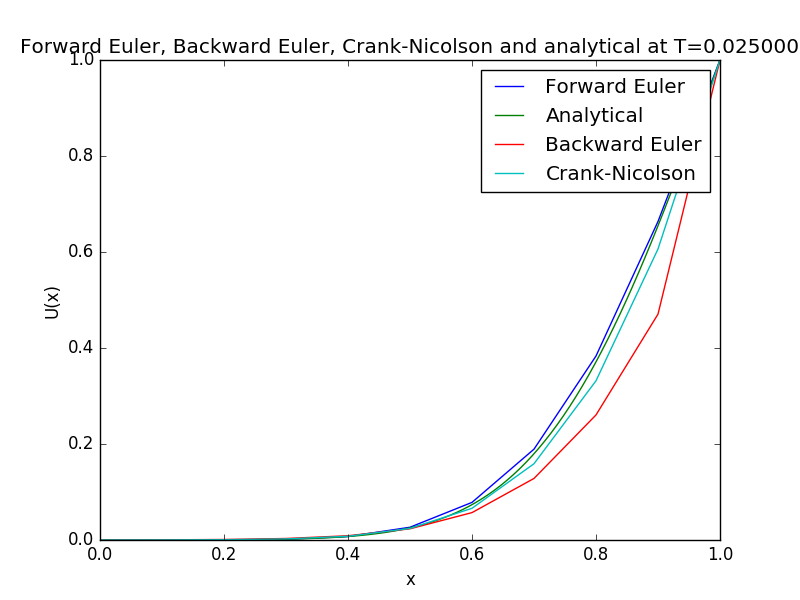
\includegraphics[scale=0.5]{alldt025analyticalt1}
    \caption{The three schemes with the analytical solutiion for when $T = 0.025$ and $dt = 0.0025$}
    \label{fig:NumAna0025}
\end{figure}

\begin{figure}
  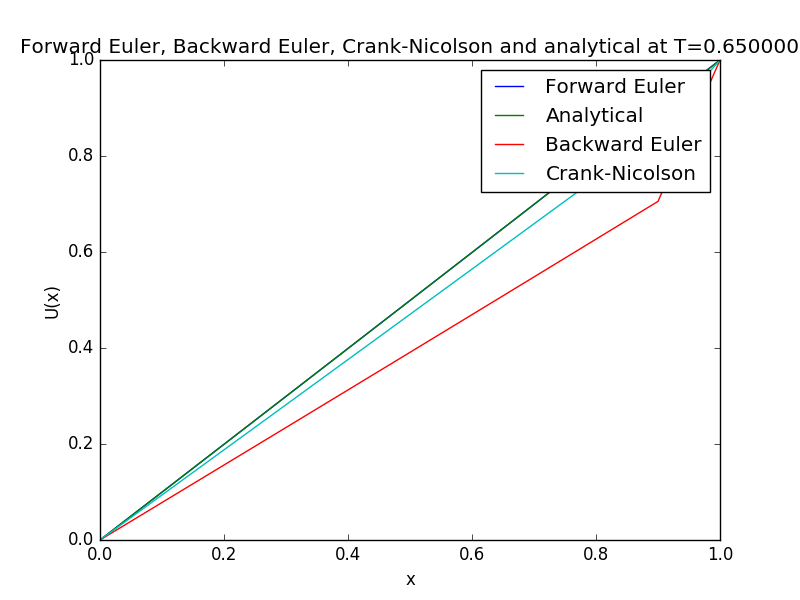
\includegraphics[scale=0.5]{alldt025analyticalt2}
    \caption{The three schemes with the analytical solutiion for when $T = 0.025$ and $dt = 0.65$}
    \label{fig:NumAna065}
\end{figure}

In figure (\ref{fig:NumAna0025}) and (\ref{fig:NumAna065}) we see the numerical calculations against the analytical for two times $t_1 = 0.025$
and $t_2 = 0.65$. And in table (\ref{tab:RelError}) we see the realtive error at the different time points. Where the relative error is
calculated with the max value and $\epsilon = |1-u_{num}/u_{anałytical}|$.

\subsection{2D PDE}
Explicit numeric solutions for different values of dx and dt are figured in plots ((\ref{fig:Num_dx0.1_dt0.0025T1}), (\ref{fig:Num_dx0.1_dt0.0025T2}), (\ref{fig:Num_dx0.1_dt0.0025T2}), (\ref{fig:Ana_dx0.1_dt0.0025T2}), (\ref{fig:Num_dx0.2}), (\ref{fig:Ana_dx0.2}), (\ref{fig:Num_alpha0.15}), (\ref{fig:Ana_alpha0.15}), (\ref{fig:Num_dx0.04}), (\ref{fig:Ana_dx0.04}), (\ref{fig:Num_feil1}), (\ref{fig:Ana_feil1}), (\ref{fig:Num_feil2}), (\ref{fig:Ana_feil2}).
\begin{figure}
  \begin{center}
    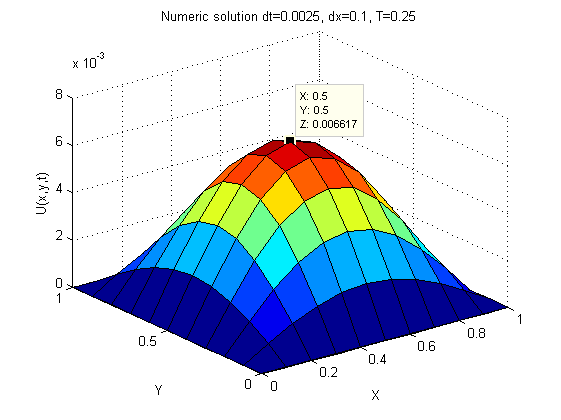
\includegraphics[scale=0.5]{num_dt00025_dx01_T025}
    \caption{Explicit solution for dx=0.1, $\alpha$ = 0.25, T=0.25}
    \label{fig:Num_dx0.1_dt0.0025T1}
  \end{center}

\end{figure}

\begin{figure}
  \begin{center}
    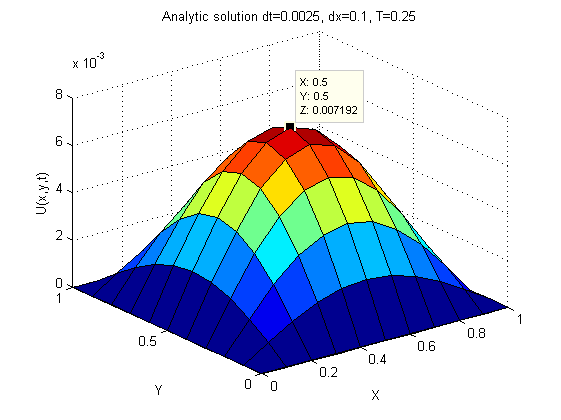
\includegraphics[scale=0.5]{ana_dt00025_dx01_T025}
    \caption{Analytical solution for dx=0.1, $\alpha$ = 0.25, T=0.25}
    \label{fig:Ana_dx0.1_dt0.0025T1}
  \end{center}
\end{figure}

\begin{figure}
  \begin{center}
    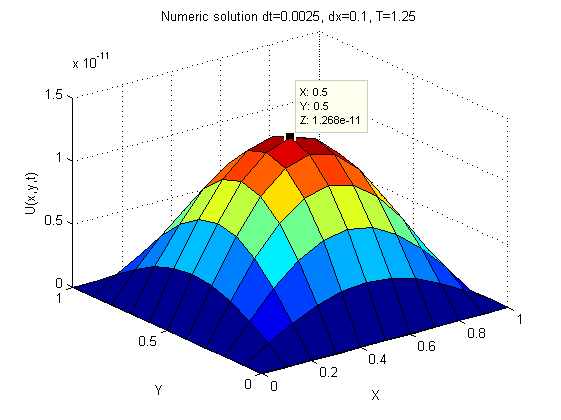
\includegraphics[scale=0.5]{num_dt00025_dx01_T125}
    \caption{Explicit solution for dx=0.1, $\alpha$ = 0.25, T=1.25}
    \label{fig:Num_dx0.1_dt0.0025T2}
  \end{center}
\end{figure}

\begin{figure}
  \begin{center}
    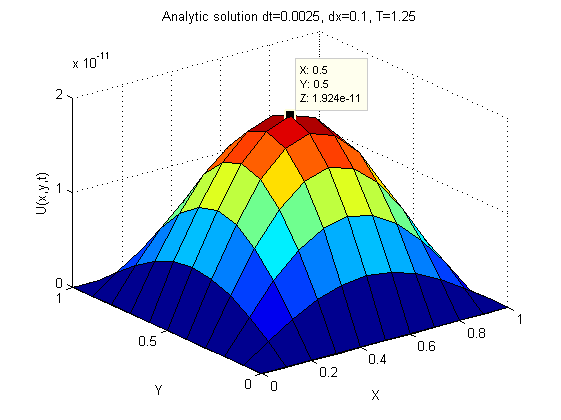
\includegraphics[scale=0.5]{ana_dt00025_dx01_T125}
    \caption{Analytical solution for dx=0.1, $\alpha$ = 0.25, T=1.25}
    \label{fig:Ana_dx0.1_dt0.0025T2}
  \end{center}
\end{figure}

\begin{figure}
  \begin{center}
    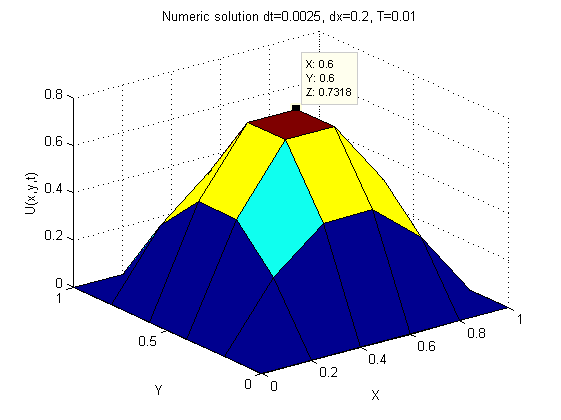
\includegraphics[scale=0.5]{num_dt00025_dx02_T001}
    \caption{Explicit solution for dx=0.2, $\alpha$ = 0.25, T=1.0}
    \label{fig:Num_dx0.2}
  \end{center}
\end{figure}

\begin{figure}
  \begin{center}
    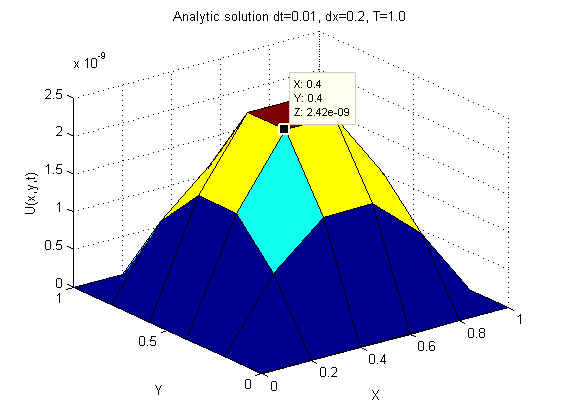
\includegraphics[scale=0.5]{ana_dt001_dx02_T10}
    \caption{Analytical solution for dx=0.2, $\alpha$ = 0.25, T=1.0}
    \label{fig:Ana_dx0.2}
  \end{center}

\end{figure}

\begin{figure}
  \begin{center}
    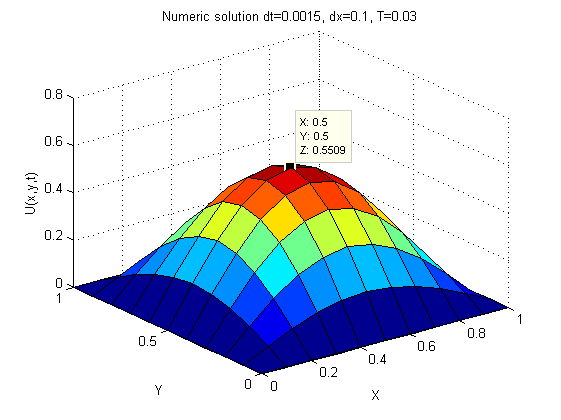
\includegraphics[scale=0.5]{num_dt00015_dx01_T003}
    \caption{Explicit solution for dx=0.1, $\alpha$ = 0.15, T=0.03}
    \label{fig:Num_alpha0.15}
  \end{center}

\end{figure}

\begin{figure}
  \begin{center}
    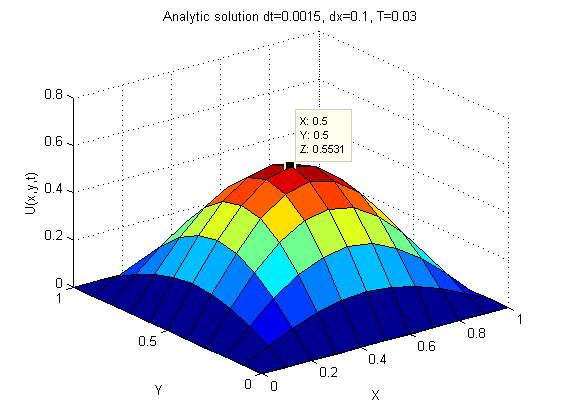
\includegraphics[scale=0.5]{ana_dt00015_dx01_T003}
    \caption{Analytical solution for dx=0.1, $\alpha$ = 0.15, T=0.03}
    \label{fig:Ana_alpha0.15}
  \end{center}

\end{figure}

\begin{figure}
  \begin{center}
    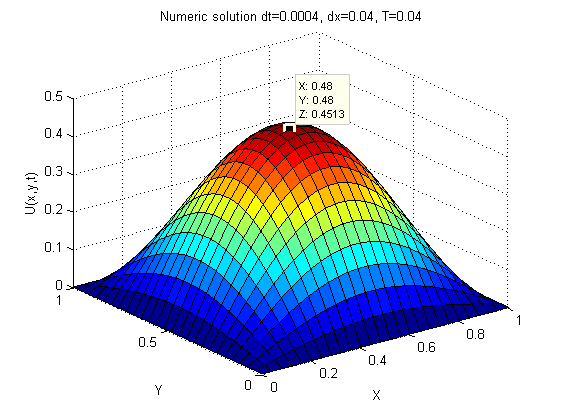
\includegraphics[scale=0.5]{num_dt00004_dx004_T004}
    \caption{Explicit solution for dx=0.04, $\alpha$ = 0.25, T=0.04}
    \label{fig:Num_dx0.04}
  \end{center}

\end{figure}
\begin{figure}
  \begin{center}
    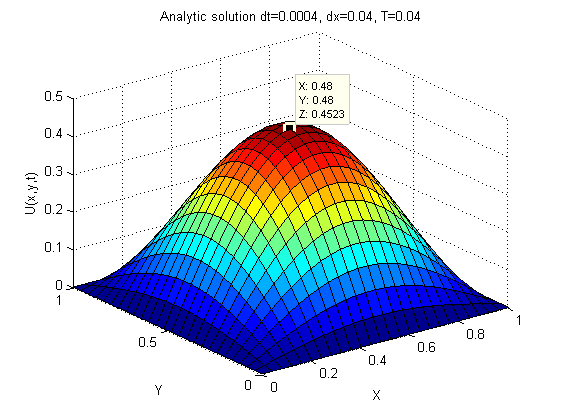
\includegraphics[scale=0.5]{ana_dt00004_dx004_T004}
    \caption{Analytic solution for dx=0.04, $\alpha$ = 0.25, T=0.04}
    \label{fig:Ana_dx0.04}
  \end{center}

\end{figure}

\begin{figure}
  \begin{center}
    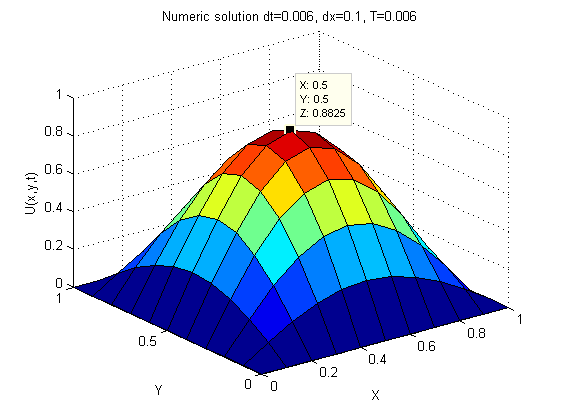
\includegraphics[scale=0.5]{num_dt0006_dx01_T0006}
    \caption{Explicit solution for dx=0.1, $\alpha$ = 0.6, T=0.006}
    \label{fig:Num_feil1}
  \end{center}

\end{figure}

\begin{figure}
  \begin{center}
    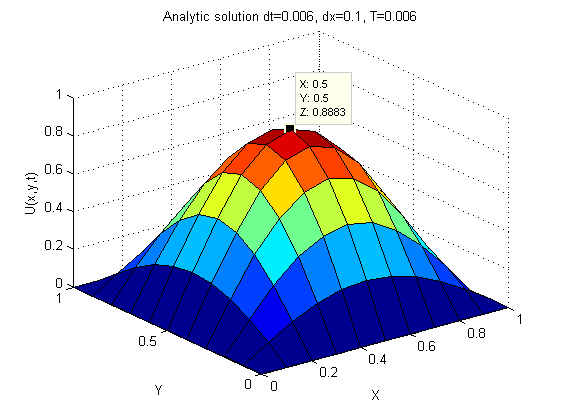
\includegraphics[scale=0.5]{ana_dt0006_dx01_T0006}
    \caption{Analytical solution for dx=0.1, $\alpha$ = 0.6, T=0.006}
    \label{fig:Ana_feil1}
  \end{center}

\end{figure}

\begin{figure}
  \begin{center}
    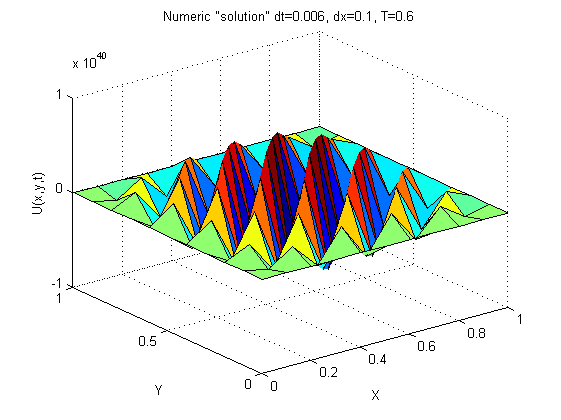
\includegraphics[scale=0.5]{num_dt0006_dx01_T06}
    \caption{Explicit solution for dx=0.1, $\alpha$ = 0.6, T=0.6}
    \label{fig:Num_feil2}
  \end{center}

\end{figure}

\begin{figure}
  \begin{center}
    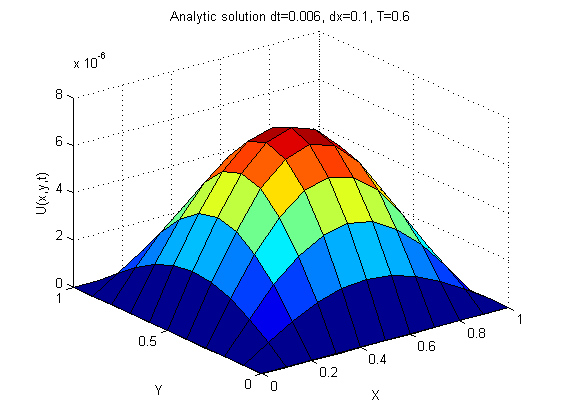
\includegraphics[scale=0.5]{ana_dt0006_dx01_T06}
    \caption{Analytical solution for dx=0.1, $\alpha$ = 0.25, T=0.6}
    \label{fig:Ana_feil2}
  \end{center}

\end{figure}

\section{Discussion}
\subsection{2D}
We see in figure (\ref{fig:NumAna0025}) that all the solutions are very correct which is not strange since it has only calculated around 10 timesteps.
But in figure (\ref{fig:NumAna065}) we see that the one that is most correct is Forward Euler, followed by Crank Nicolson and lastly Backward Euler. 
Yo can see the relative errors in the table (\ref{tab:RelError}), for these plots we have used as stated before the timestep: $\Delta t = 0.0025$.
So the truncation error in Forward and Backward euler is both $\epsilon = 0.0025$ and in Crank Nicolson it is $\epsilon = 6.25*10^{-6}$. 
Since the truncation error is the error committed by one step of the method, and it assumes the earlier step is the exact solution it will be an accumulated error.
But in our plot (figure (\ref{fig:NumAna065}) we see that the Forward Euler method is incredible correct. This is because of the initial values are  

\subsection{3D}

\section{Conclusion}

\section{Codes}

\section{Sources}

\end{document}
